\documentclass[12pt]{article}

\usepackage[utf8]{inputenc}
\usepackage{svg}
\usepackage[T1]{fontenc}
\usepackage[english]{babel}
\usepackage{tabularx}
\usepackage{hyperref}
\usepackage[margin=2cm,a4paper,headsep=1.2cm]{geometry}
\usepackage{ifthen}
\usepackage{fancyhdr}
\usepackage{tikz}
\usetikzlibrary{arrows}
\usetikzlibrary{arrows.meta}

\renewcommand{\baselinestretch}{1.1}
\setlength{\parindent}{0pt}
\setlength{\parskip}{1em}

\setlength{\headheight}{1cm}
\setlength{\headwidth}{\textwidth}

\makeatletter
\newcommand{\labeltext}[2]{%
  \@bsphack
  \csname phantomsection\endcsname % in case hyperref is used
  \def\@currentlabel{#1}{\label{#2}}%
  \@esphack
}
\makeatother    

\newcommand{\prio}[1]{\ifthenelse{\equal{#1}{1}}{low}{\ifthenelse{\equal{#1}{2}}{medium}{\ifthenelse{\equal{#1}{3}}{high}{\textbf{INVALID!}}}}\relax}

\newcounter{fr}
\newcommand{\fr}[8]{
\refstepcounter{fr}\label{#8}
\begin{tabularx}{16cm}{l|X}
 & \textbf{#1} \hfill \textbf{FR\arabic{fr}} \\ \hline
Description & #2\\ \hline
\ifthenelse{\equal{#3}{}}{}{Precondition & #3 \\ \hline}
\ifthenelse{\equal{#4}{}}{}{Postcondition & #4 \\ \hline}
Rationale & #5
\ifthenelse{\equal{#6}{}}{}{\\ \hline Dependencies & #6} 
\ifthenelse{\equal{#7}{}}{}{ \\ \hline Priority & \prio{#7}}
\end{tabularx}
\vspace*{0.75cm}
}

\newcommand{\actor}[4]{
\labeltext{#2}{#1}
\begin{tabularx}{16cm}{|l|X|}
\hline 
Actor: & #2 \\
\hline
Description: & #3 \\
\hline
Representative: & #4 \\
\hline
\end{tabularx}
}

%\newcommand{\rref}[1]{\ref{#1}\textsuperscript{$\rightarrow$ p. \pageref{#1}}}
\newcommand{\rref}[1]{\ref{#1}}
\newcommand{\frref}[1]{FR\ref{#1}\textsuperscript{$\rightarrow$ p. \pageref{#1}}}
\newcommand{\nfrref}[1]{QR\ref{#1}\textsuperscript{$\rightarrow$ p. \pageref{#1}}}

\newcommand{\myrule}[1]{
	\begin{tikzpicture}
		\draw[{Diamond[open]}-{Diamond[open]}, ultra thick] (0,0) to (#1, 0);
	\end{tikzpicture}
}

\renewcommand{\contentsname}{Table of Contents}

\begin{document}

% title page 
\begin{titlepage}

	\centering 
	\scshape 
	\vspace*{\baselineskip}
		
	\myrule{\linewidth}	
	\rule[1\baselineskip]{0.95\textwidth}{0.4pt}
    
    \Large
    Design Documentation
    \normalsize
   

	\rule[-1\baselineskip]{0.95\textwidth}{0.4pt}
	\myrule{\linewidth}
	
	\vspace{2\baselineskip}

    Flutter smart sensing library \\ for medical and psychological study apps
	
	
	\vspace*{15\baselineskip}
	
	edited by
	
	\vspace{0.55\baselineskip}
	
	{\scshape Leonhard Alkewitz, Florian Gebhardt, Hermann Fröhlich, \\ Mukhtar Muse, Felix Schlegel}
	
	\vspace{0.55\baselineskip}
	
	\vfill
	
\end{titlepage}


% table of contents
\tableofcontents
\thispagestyle{empty}

\newpage

% configure header and footer
\pagestyle{fancy}

\fancyhead[R]{\thepage}
\fancyhead[L]{\leftmark}
\fancyfoot{}

\section{Introduction}
\label{sec:Intro}
This document lists all the architectures for the Flutter Smart Sensing Library. Each diagram includes a description of why it was designed in that way and why certain changes were necessary. Every change is listed in this document.
\section{Software Architecture}
This section covers the software architecture. It is split into two core components: the \hyperref[sec:SmartSensingLibrary]{Smart Sensing Library} and the \hyperref[sec:SensingPlugin]{Sensing Plugin}. The reason for this is that we have one component to read and standardize sensor data in a platform-independent way, while the other component represents most of the smart features like storage and filtering of values.

\subsection{Smart Sensing Library}
\label{sec:SmartSensingLibrary}
The Smart Sensing Library contains most of the features requested by the customer. It serves as the access point to read sensor data. Its design is inspired by the pipe and filter architecture. That way the customer can chain different filters on one dataset. The library is split into three main components: \hyperref[sec:BufferManager]{BufferManager}, \hyperref[sec:FilterTools]{FilterTools}, and API. The API has all public methods that can be used by the customer to subscribe to sensors and retrieve filtered sensor data. The \hyperref[sec:BufferManager]{BufferManager} is responsible for managing all sensor data streams and writing them into the database. It also contains a buffer cache for faster access times. The \hyperref[sec:FilterTools]{FilterTools} are used to apply different filters to the sensor data.

%Explaination for Storage plugin is missing%
\subsubsection{Version 1}
\begin{figure}[ht]
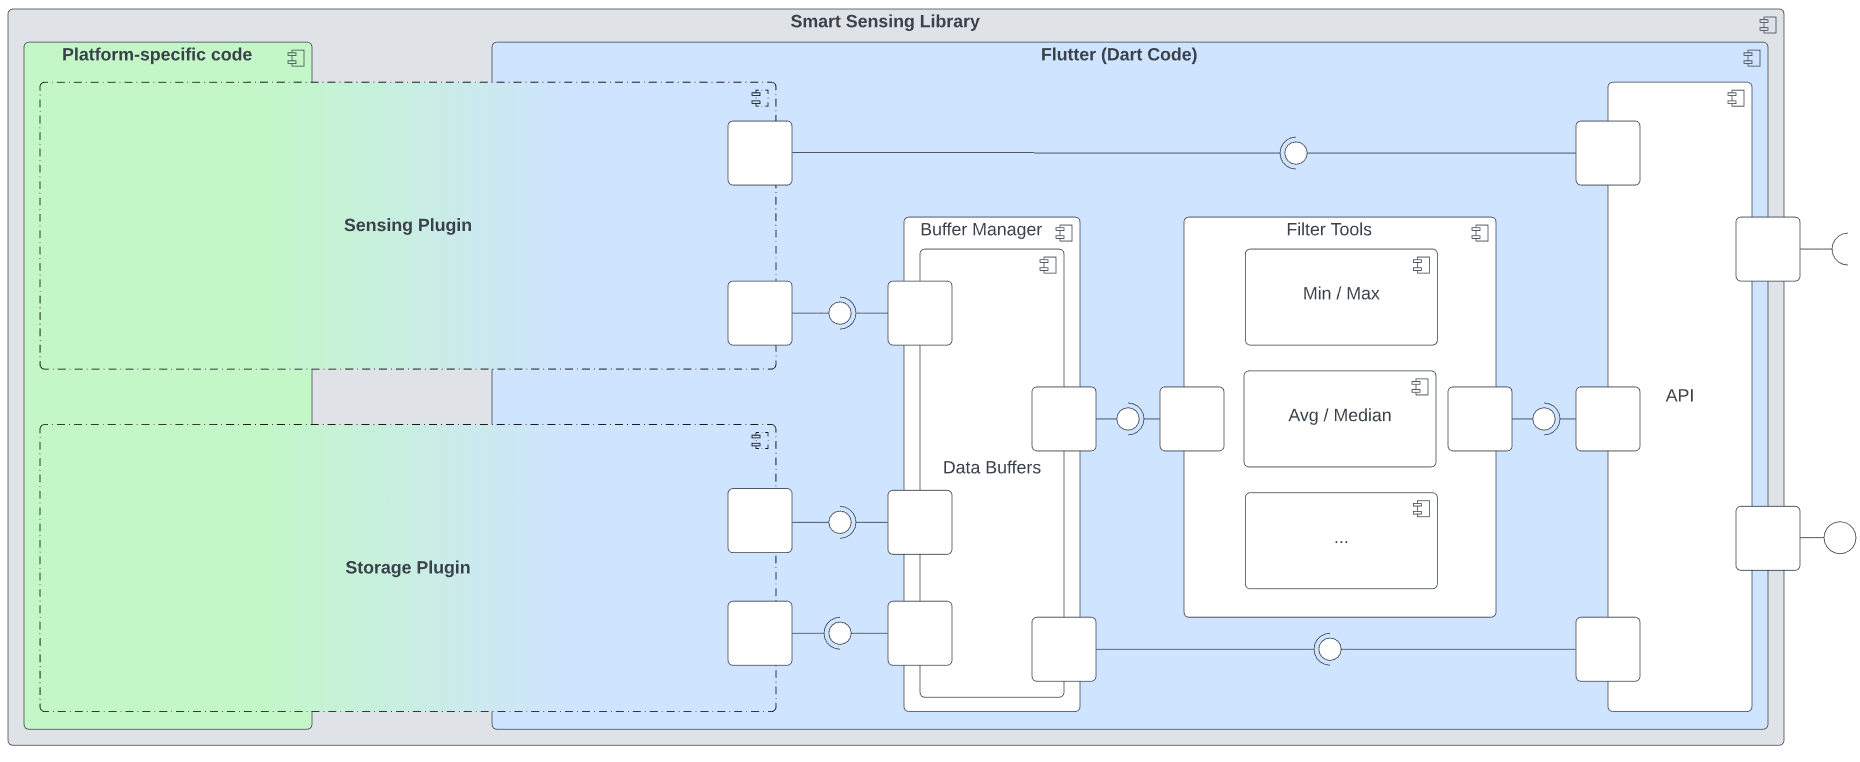
\includegraphics[width=1\textwidth]{Graphics/SmartSensingLibraryOld.png}
\caption{\label{fig:bild1}Version 1.0}
\end{figure}
\subsubsection{Version 1.1}
An architectural change was made where the \hyperref[sec:BufferManager]{BufferManager} and \hyperref[sec:FilterTools]{FilterTools} were incorporated into a new component called \hyperref[sec:IOManager]{IOManager}.
The reason for this change is that the coordination between the API, \hyperref[sec:FilterTools]{FilterTools}, and \hyperref[sec:BufferManager]{BufferManager} was not considered while creating the first iteration. The \hyperref[sec:CIOManager]{IOManager} is now the primary communication point between the API and the underlying services.
\begin{figure}[ht]
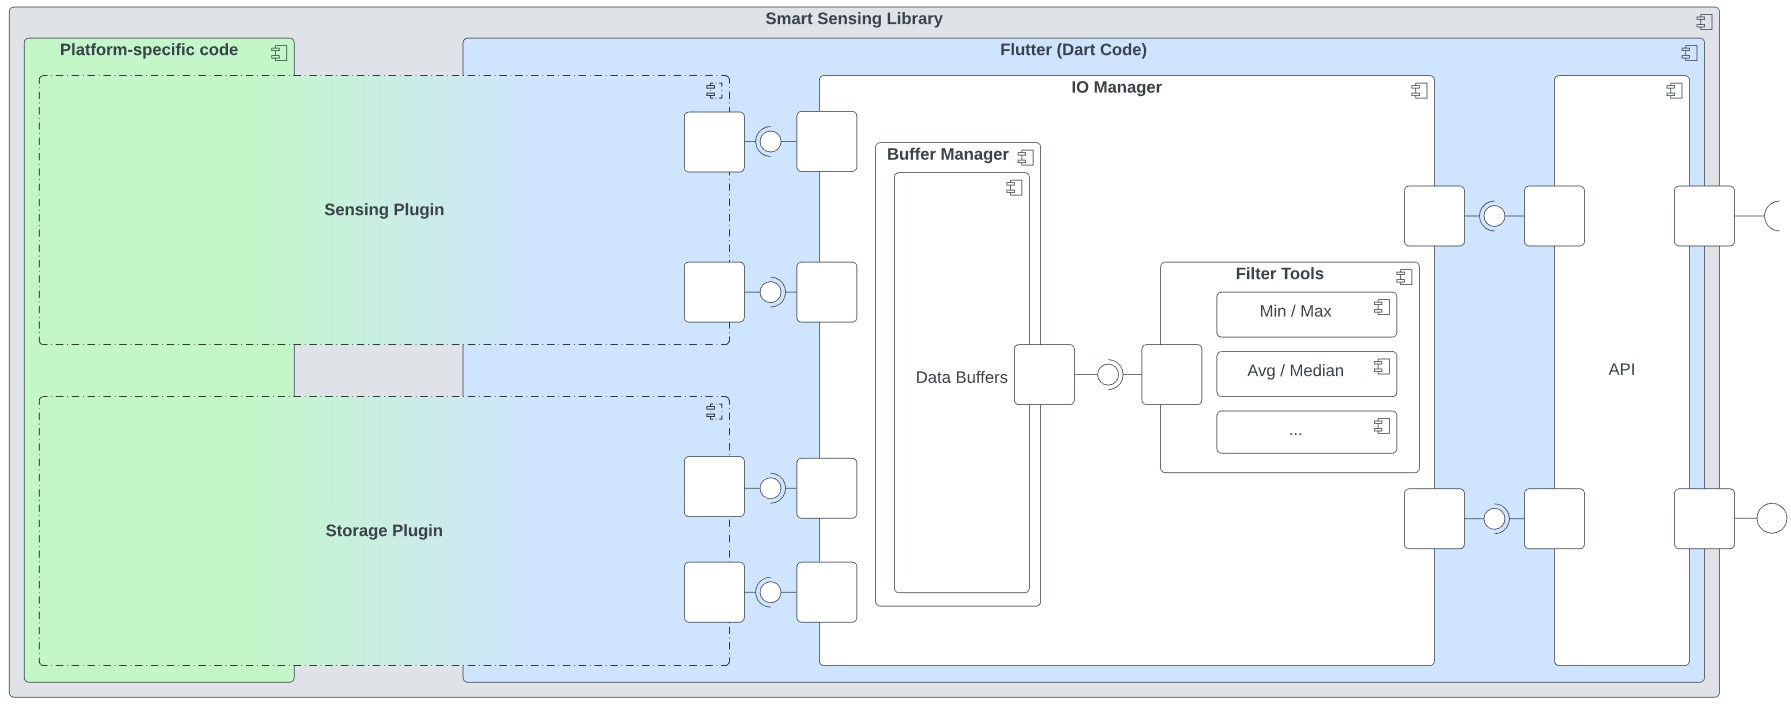
\includegraphics[width=1\textwidth]{Graphics/SmartSensingLibraryNew.png}
\caption{\label{fig:bild2} Version 1.1}
\end{figure}
\newpage
\subsection{Sensing Plugin}
\label{sec:SensingPlugin}
The Sensing Plugin is responsible for reading sensor data from iOS and Android devices and performing pre-processing on the data. This standardizes the data and allows the customer to apply various configurations. It's split into two main parts: the platform-specific code and the Dart code. The platform-specific code is responsible for reading sensor data from the device using factory methods provided by the corresponding operating system. These methods can then be called by the Dart code using method channels. In the Dart code, the data is unified (e.g. unit, decimal precision and axis orientation) so that the \hyperref[sec:SmartSensingLibrary]{Smart Sensing Library} can work with the data. The \hyperref[sec:CSensorManager]{SensorManager} has two main components. The Command Caller is responsible for delegating customer request like sensor subscription. The Sensor Event Subscriber handels the return of the subscriptions.
\subsubsection{Version 1}
\begin{figure}[ht]
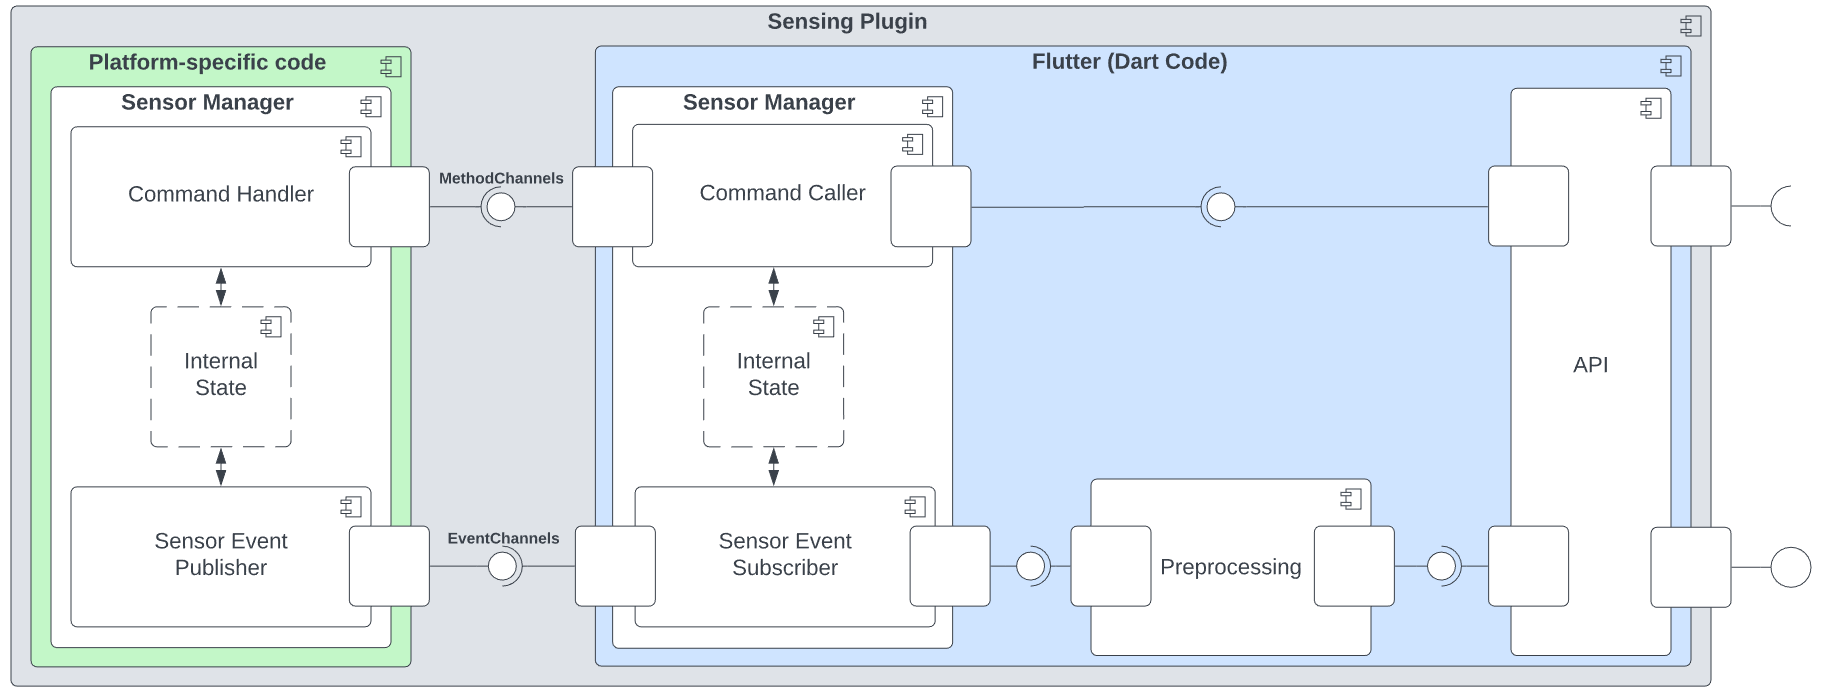
\includegraphics[width=1\textwidth]{Graphics/SmartSensingPluginOld.png}
\caption{\label{fig:bild3} Version 1.0}
\end{figure}

\subsubsection{Version 1.1}
There was an architectural change made where the pre-processing is now part of the \hyperref[sec:SensorManager]{SensorManager}. The reason for this change is that the \hyperref[sec:Preprocessor]{preprocessor} should be a component for the \hyperref[sec:SensorManager]{SensorManager} to use. In the first iteration, the \hyperref[sec:Preprocessor]{preprocessor} was seen as a single instance that would process all data, but it was later reconsidered that it would be more beneficial to use one \hyperref[sec:Preprocessor]{preprocessor} for each sensor. This allows for easier configuration of each sensor's output.
\begin{figure}[ht]
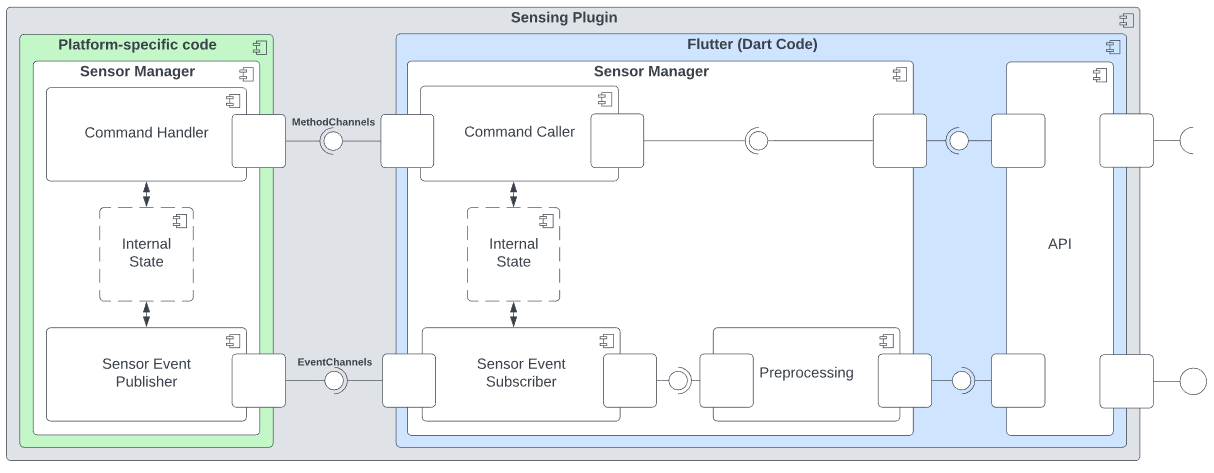
\includegraphics[width=1\textwidth]{Graphics/SmartSensingPluginNew.png}
\caption{\label{fig:bild4} Version 1.1}
\end{figure}

\newpage
\section{Class Diagramms}
\label{sec:ClassDiagramms}
This section covers the class diagrams for each component. Each diagram includes a description of the design choices made for that component.

\subsection{IOManager}
\label{sec:CIOManager}
The IOManager component manages all functions related to data storage and transfer. It is the main component for the \hyperref[sec:SmartSensingLibrary]{Smart Sensing Library}.
\begin{figure}[ht]
\centering
\includesvg[width=1\textwidth]{Graphics/CIOManager}
\caption{\label{fig:bild5} IOManager Component Version 1.0}
\end{figure}

\begin{figure}[ht]
\centering
\includesvg[width=1\textwidth]{Graphics/CIOManagerUpdated}
\caption{\label{fig:bild6} IOManager Component Version 1.1}
\end{figure}


\subsubsection{IOManager}
\label{sec:IOManager}
The IOManager is implemented using the Singleton pattern. The reason for this is that sensor data should be controlled by only one component, not multiple, to prevent multiple access to data streams. There is always only one IOManager present in the \hyperref[sec:SmartSensingLibrary]{Smart Sensing Library}. It controls all data operations related to sensor data.
\begin{figure}[ht]
\centering
\includesvg[width=.6\textwidth]{Graphics/IOManager}
\caption{\label{fig:bild7} IOManager Version 1.0}
\end{figure}

The updated version represents the current implementation. It is more detailed and also adds new functionalities to the IOManager. Added functionalities are:   
\begin{itemize}
  \item Import and export of data.
  \item Information about the current \hyperref[sec:SensorManager]{SensorManager} state.
  \item Internal sensor stream handling.
  \item Internal redesigning for testing purposes. 
\end{itemize}


\begin{figure}[ht]
\centering
\includesvg[width=.6\textwidth]{Graphics/IOManagerUpdated}
\caption{\label{fig:bild8} IOManager Version 1.1}
\end{figure}

\subsubsection{BufferManager}
\label{sec:BufferManager}
The BufferManager class functions as a cache for currently used data. All new data is first saved into its buffer. If it becomes full, the \hyperref[sec:IOManager]{IOManager} takes its current content and saves it to the database if necessary. The Buffer Manager only contains sensor data that hasn't been modified by filters, this way the data can be reused by different functions.
\begin{figure}[ht]
\centering
\includesvg[width=0.6\textwidth]{Graphics/BufferManager}
\caption{\label{fig:bild9} BufferManager Version 1.0}
\end{figure}
\newpage

The updated version represents the current implementation. It is more detailed and adds a sorting functionality.

\begin{figure}[ht]
\centering
\includesvg[width=0.5\textwidth]{Graphics/BufferManagerUpdated}
\caption{\label{fig:bild10} BufferManager Version 1.1}
\end{figure}


\subsubsection{FilterTools}
\label{sec:FilterTools}
The FilterTools are used to modify the data from the \hyperref[sec:BufferManger]{BufferManager} by deep-copying the needed values. After the initial copy, filters can be chained to create more complex queries. The FilterTools provide the only means for accessing the data.
\begin{figure}[ht]
\centering
\includesvg[width=0.5\textwidth]{Graphics/FilterTools}
\caption{\label{fig:bild11} FilterTools Version 1.0}
\end{figure}
\newpage

The updated version represents the current implementation. It now works with the flutter internal \hyperlink{https://flutterbyexample.com/lesson/cascade-notation}{cascade} function. It also added the functionality to set a specific time intervall, in which the data is filtered (eg. the average every day). 
\begin{figure}[ht]
\centering
\includesvg[width=0.6\textwidth]{Graphics/FilterToolsUpdated}
\caption{\label{fig:bild12} FilterTools Version 1.1}
\end{figure}

\subsubsection{MultiFilterTools}
\label{sec:MultiFilterTools}
The MultiFilterTools extend the \hyperref[sec:FilterTools]{FilterTools} and was added with version 1.1. It added the functionality to create a query on multiple sensors simultaneously. 
\begin{figure}[ht]
\centering
\includesvg[width=0.6\textwidth]{Graphics/MultiFilterTools}
\caption{\label{fig:bild13} MultiFilterTools}
\end{figure}
\newpage

\subsubsection{DeviceInformationManager}
\label{sec:DeviceInformationManager}
The device information manager was added with Version 1.1. It added the functionality to read current device information, like current OS or free space.
\begin{figure}[ht]
\centering
\includesvg[width=0.6\textwidth]{Graphics/DeviceInformationManager}
\caption{\label{fig:bild14} DeviceInformationManager}
\end{figure}


\subsubsection{SensorDataDTO}
\label{sec:SensorDataDTO}
The SensorDataDTO was added with version 1.1. It serves as the SensorData datatype in the database. The reason for the seperation between SensorDataDTO and \hyperref[sec:SensorData]{SensorData} is the mutable state. SensorDataDTO is immutable while \hyperref[sec:SensorData]{SensorData} can get changed (e.g. by the preprocessor) and is therefore mutable. The immutable state is needed for the database. DTO stands for "Data Transfer Object".

\begin{figure}[ht]
\centering
\includesvg[width=0.6\textwidth]{Graphics/SensorDataDTO}
\caption{\label{fig:bild15} SensorDataDTO}
\end{figure}
\newpage


\subsubsection{Import/Export Module}
\label{sec:Import/ExportModule}
The Import/Export module was added with version 1.1. It added the functionality to import or export data to and from the database. It consists of three objects:
\begin{itemize}
  \item The ImportModule, which handles all import functions.
  \item The ExportModule, which handles all export functions.
  \item The SupportedFileFormats, which represent all supported file formats.
\end{itemize}

\begin{figure}[ht]
\centering
\includesvg[width=0.5\textwidth]{Graphics/ImportModule}
\caption{\label{fig:bild16} ImportModule}
\end{figure}

\begin{figure}[ht]
\centering
\includesvg[width=0.5\textwidth]{Graphics/ExportModule}
\caption{\label{fig:bild17} ExportModule}
\end{figure}

\begin{figure}[ht]
\centering
\includesvg[width=0.4\textwidth]{Graphics/SupportedFormat}
\caption{\label{fig:bild18} SupportedFileFormats}
\end{figure}

\newpage
\null
\newpage

\subsection{SensorManager}
\label{sec:CSensorManager}
The SensorManager component serves as the interface between Dart code and platform-specific code. It offers the ability to subscribe and unsubscribe to sensor data streams, which implements the pub/sub pattern. It also preprocesses the data to ensure that Android and iOS return consistent target units. The preprocessing can be configured as needed.
\begin{figure}[ht]
\centering
\includesvg[width=1\textwidth]{Graphics/CSensorManager}
\caption{\label{fig:bild19} SensorManager Component Version 1.0}
\end{figure}
\newpage

The updated version represents the current implementation. It is more detailed and also adds new functionalities to the IOManager. Added functionalities are:   
\begin{itemize}
  \item Import and export of data.
  \item Information about the current \hyperref[sec:SensorManager]{SensorManager} state.
  \item Internal sensor stream handling.
  \item Internal redesigning for testing purposes. 
\end{itemize}

\begin{figure}[ht]
\includesvg[width=1\textwidth]{Graphics/CSensorManagerUpdated}
\caption{\label{fig:bild20} SensorManager Component Version 1.1}
\end{figure}
\newpage

\subsubsection{SensorManager}
\label{sec:SensorManager}
The SensorManager class is the central control unit for the component and follows the singleton design pattern. It manages all aspects related to subscribing and unsubscribing to sensors and delegates these requests to the platform-specific code, which then returns the corresponding responses.
\begin{figure}[ht]
\centering
\includesvg[width=0.6\textwidth]{Graphics/Sensormanager}
\caption{\label{fig:bild21} SensorManager}
\end{figure}

\subsubsection{Sensor}
\label{sec:Sensor}
This class is representing a sensor.
\begin{figure}[ht]
\centering
\includesvg[width=0.6\textwidth]{Graphics/Sensor}
\caption{\label{fig:bild22} Sensor}
\end{figure}
\newpage

\subsubsection{SensorPropertyValidator}
\label{sec:SensorPropertyValidator}
The SensorPropertyValidator class ensures that the specified precision and time intervall are maintained.
\begin{figure}[ht]
\centering
\includesvg[width=0.6\textwidth]{Graphics/SensorPropertyValidator}
\caption{\label{fig:bild23} SensorPropertyValidator}
\end{figure}


\subsubsection{Preprocessor}
\label{sec:Preprocessor}
The Peprocessor class ensures that Android and iOS return consistent value types. It can be configured with the \hyperref[sec:SensorConfig]{SensorConfig}.
\begin{figure}[ht]
\centering
\includesvg[width=0.6\textwidth]{Graphics/PreProcessor}
\caption{\label{fig:bild24} Preprocessor}
\end{figure}
\newpage
\subsubsection{SensorConfig}
\label{sec:SensorConfig}
The SensorConfig class holds various configurations for the \hyperref[sec:Preprocessor]{preprocessor}, including the time intervall, precision, and target unit.
\begin{figure}[ht]
\centering
\includesvg[width=0.6\textwidth]{Graphics/SensorConfig}
\caption{\label{fig:bild25} SensorConfig}
\end{figure}


\subsubsection{SensorDataSubscriber}
\label{sec:SensorDataSubscriber}
The SensorDataSubscriber class manages multiple subscriptions and is utilized by the \hyperref[sec:CSensorManager]{SensorManager} class.
\begin{figure}[ht]
\centering
\includesvg[width=0.6\textwidth]{Graphics/DataSubscriber}
\caption{\label{fig:bild26} SensorDataSubscriber}
\end{figure}
\newpage
\subsubsection{SensorData}
\label{sec:SensorData}
The SensorData class represents the data received from a sensor and serves as the data model for the document-based database.
\begin{figure}[ht]
\centering
\includesvg[width=0.6\textwidth]{Graphics/SensorData}
\caption{\label{fig:bild27} SensorData}
\end{figure}
\newpage

\section{Processes}
\label{sec:Processes}
\subsection{Sequence Diagrams}
This section contains sequence diagrams for getting and modifying data.

\subsubsection{Starting a Sensor}
\label{sec:StartingASensor}
\begin{figure}[ht]
\centering
\includesvg[width=0.6\textwidth]{Graphics/AddSensor}
\caption{\label{fig:bild28} Starting a Sensor}
\end{figure}

\newpage


\subsubsection{Removing a Sensor}
\label{sec:RemovingASensor}
\begin{figure}[ht]
\centering
\includesvg[width=0.6\textwidth]{Graphics/RemoveSensor}
\caption{\label{fig:bild29} Removing a Sensor}
\end{figure}


\subsubsection{Getting a filter}
\label{sec:GettingAFilter}
\begin{figure}[ht]
\centering
\includesvg[width=0.7\textwidth]{Graphics/GetFilterData}
\caption{\label{fig:bild30} Getting a filter}
\end{figure}
\end{document}